%QUESTIONS HERE
%<*mytag1>
\begin{questions}[resume,start=\number\value{questionsi}+1,noitemsep,leftmargin=20mm,labelsep=0.1cm]
\item What is gcc?
\end{questions}
%</mytag1>

%<*mytag2>
\begin{questions}[resume,start=\number\value{questionsi}+1,noitemsep,leftmargin=20mm,labelsep=0.1cm]
\item What does the \texttt{--prefix} option do?
\end{questions}
%</mytag2>

%<*mytag3>
\begin{questions}[resume,start=\number\value{questionsi}+1,noitemsep,leftmargin=20mm,labelsep=0.1cm]
\item Compare the permissions under each ACL group.
\end{questions}
%</mytag3>

%<*mytag4>
\begin{questions}[resume,start=\number\value{questionsi}+1,noitemsep,leftmargin=20mm,labelsep=0.1cm]
\item Which commands for the sys\textunderscore admin group are only allowed with certain options?
\end{questions}
%</mytag4> 

%<*mytag5>
\begin{questions}[resume*,start=\number\value{questionsi}+1,noitemsep,leftmargin=20mm,labelsep=0.1cm]
\item What is the difference between the \texttt{login} and \texttt{enable} password fields?
\end{questions}
%</mytag5> 

%<*mytag6>
\begin{questions}[resume,start=\number\value{questionsi}+1,noitemsep,leftmargin=20mm,labelsep=0.1cm]
\item 
\item
\end{questions}
%</mytag6> 

%<*mytag7>
\begin{questions}[resume*,start=\number\value{questionsi}+1,noitemsep,leftmargin=20mm,labelsep=0.1cm]
\item 
\item
\end{questions}
%</mytag7>

%<*mytag8>
\begin{questions}[resume,start=\number\value{questionsi}+1,noitemsep,leftmargin=20mm,labelsep=0.1cm]
\item 
\item
\end{questions}
%</mytag8>

%<*mytag9>
\begin{questions}[resume,start=\number\value{questionsi}+1,noitemsep,leftmargin=20mm,labelsep=0.1cm]
\item 
\item
\end{questions}
%</mytag9>

%LISTS HERE

%<*mytag10>
\begin{enumerate}[noitemsep,label=$\circ$,leftmargin=17mm,labelsep=0.5cm]
\item
\item
\end{enumerate}
%</mytag10>

%<*mytag11>
\begin{enumerate}[noitemsep,leftmargin=10mm,labelsep=0.1cm]
\item Test item
\item
\end{enumerate}
%</mytag11>


%COMMANDS HERE
%<*mytag12>
\begin{enumerate}[noitemsep,leftmargin=10mm,labelsep=0.1cm]
\item [] \textbf{wget ftp://ftp.shrubbery.net/pub/tac\textunderscore plus/tacacs+-F4.0.4.26.tar.gz && tar zxvf tacacs+-F4.0.4.26.tar.gz}
\end{enumerate}
%</mytag12>

%<*mytag13>
\begin{enumerate}[noitemsep,leftmargin=10mm,labelsep=0.1cm]
\item [] \textbf{dpkg -s gcc bison flex}
\end{enumerate}
%</mytag13>
%<*mytag14>
\begin{enumerate}[noitemsep,label=$\circ$,leftmargin=17mm,labelsep=0.5cm]
\item [] \textbf{./configure -help}
\end{enumerate}
%</mytag14>
%<*mytag15>
\begin{enumerate}[noitemsep,leftmargin=10mm,labelsep=0.1cm]
\item [] \textbf{./configure --enable-acls --enable-uenable && make install}
\end{enumerate}
%</mytag15>
%<*mytag16>
\begin{enumerate}[noitemsep,leftmargin=10mm,labelsep=0.1cm]
\item [] \textbf{tac\_pwd}
\end{enumerate}
%</mytag16>
%<*mytag17>
\begin{enumerate}[noitemsep,leftmargin=10mm,labelsep=0.1cm]
\item [] \textbf{Password to be encrypted: \<your password here\>}
\end{enumerate}
%</mytag17>
%<*mytag18>
\begin{enumerate}[noitemsep,leftmargin=10mm,labelsep=0.1cm]
\item [] \textbf{touch /etc/default/tac\textunderscore plus}
\end{enumerate}
%</mytag18>
%<*mytag19>
\begin{enumerate}[noitemsep,leftmargin=10mm,labelsep=0.1cm]
\item [] \textbf{chmod 755 /etc/default/tac\textunderscore plus}
\end{enumerate}
%</mytag19>
%<*mytag20>
\begin{enumerate}[noitemsep,leftmargin=10mm,labelsep=0.1cm]
\item [] \textbf{nano /etc/default/tac\textunderscore plus}
\end{enumerate}
%</mytag20>
%<*mytag21>
\begin{enumerate}[noitemsep,leftmargin=10mm,labelsep=0.1cm]
\item [] \textbf{/etc/init.d/tac\textunderscore plus start}
\end{enumerate}
%</mytag21>
%<*mytag22>
\begin{enumerate}[noitemsep,leftmargin=10mm,labelsep=0.1cm]
\item [] \textbf{ps aux | grep tac\textunderscore plus} 
\end{enumerate}
%</mytag22>
%<*mytag23>
\begin{enumerate}[noitemsep,leftmargin=10mm,labelsep=0.1cm]
\item [] \textbf{netstat -an | grep :49}
\end{enumerate}
%</mytag23>
%<*mytag24>
\begin{enumerate}[noitemsep,leftmargin=10mm,labelsep=0.1cm]
\item [] \textbf{services}
\end{enumerate}
%</mytag24>
%<*mytag25>
\begin{enumerate}[noitemsep,leftmargin=10mm,labelsep=0.1cm]
\item [] \textbf{vulns}
\end{enumerate}
%</mytag25>
%<*mytag26>
\begin{enumerate}[noitemsep,leftmargin=10mm,labelsep=0.1cm]
\item [] \textbf{db\_import $<$name of the Nessus scan file including path$>$}
\end{enumerate}
%</mytag26>
%<*mytag27>
\begin{enumerate}[noitemsep,leftmargin=10mm,labelsep=0.1cm]
\item [] \textbf{vulns}
\end{enumerate}
%</mytag27>

%<*mytag28>
\begin{enumerate}[noitemsep,label=$\circ$,leftmargin=14mm,labelsep=0.5cm]
\item Find Metasploit source code of the exploit CVE-2007-2447.  Find out the different payloads available, if any!  What programming language is it written in?  Provide a copy of the source code and explain what the code does.  Hint: it is a short script!
\item From the Wireshark capture in Step 2, find the specific set of packets exchanged between Nessus and Metasploitable2 that led Nessus to identify samba username vulnerability. Provide a pcap export of these packets and explain the algorithm used. 
\item \hl{Clone Nexpose VM (this is an open source equivalent to Nessus) and generate a vulnerability report on Metasploitable2.  Compare the results of Nessus and Nexpose in terms of the number of and the specific vulnerabilities identified.}
\end{enumerate}
%</mytag28>


%GRAPHICS HERE

%<*mtag1>
\begin{figure}[H]
\centering
\captionsetup{width=.8\linewidth}
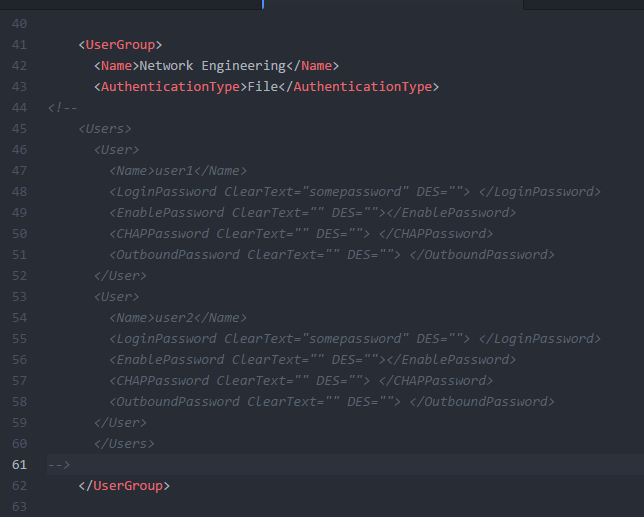
\includegraphics[scale=0.9]{img/8_commentusers.PNG}
\caption{}
\label{fig:1}
\centering
\end{figure}
%</mtag1>

%<*mtag2>
\begin{figure}[H]
\centering
\captionsetup{width=.8\linewidth}
\includegraphics[scale=0.9]{img/.png}
\caption{}
\label{fig:2}
\centering
\end{figure}
%</mtag2>

%<*mtag3>
\begin{figure}[H]
\centering
\captionsetup{width=.8\linewidth}
\includegraphics[scale=0.9]{img/.png}
\caption{}
\label{fig:3}
\centering
\end{figure}
%</mtag3>